% \iffalse
\let\negmedspace\undefined
\let\negthickspace\undefined
\documentclass[journal,12pt,twocolumn]{IEEEtran}
\usepackage{amssymb}
\usepackage{cite}
\usepackage{amsmath,amssymb,amsfonts,amsthm}
\usepackage{algorithmic}
\usepackage{graphicx}
\usepackage{textcomp}
\usepackage{xcolor}
\usepackage{txfonts}
\usepackage{listings}
\usepackage{enumitem}
\usepackage{mathtools}
\usepackage{gensymb}
\usepackage{comment}
\usepackage[breaklinks=true]{hyperref}
\usepackage{tkz-euclide} 
\usepackage{listings}
\usepackage{gvv}                                        
\def\inputGnumericTable{}                                 
\usepackage[latin1]{inputenc}                                
\usepackage{color}                                            
\usepackage{array}                                            
\usepackage{longtable}                                       
\usepackage{calc}                                             
\usepackage{multirow}                                         
\usepackage{hhline}                                           
\usepackage{ifthen}                                           
\usepackage{lscape}
\usepackage{pgfplots}
\newtheorem{theorem}{Theorem}[section]
\newtheorem{problem}{Problem}
\newtheorem{proposition}{Proposition}[section]
\newtheorem{lemma}{Lemma}[section]
\newtheorem{corollary}[theorem]{Corollary}
\newtheorem{example}{Example}[section]
\newtheorem{definition}[problem]{Definition}
\newcommand{\BEQA}{\begin{eqnarray}}
\newcommand{\EEQA}{\end{eqnarray}}
\newcommand{\define}{\stackrel{\triangle}{=}}
\theoremstyle{remark}
\newtheorem{rem}{Remark}
\begin{document}

\bibliographystyle{IEEEtran}
\vspace{3cm}

\title{GATE 2023-BM.54}
\author{EE22BTECH11004 - Allu Lohith}

\maketitle

    A system is described by the following differential equation
    
    $$\brak{0.01} \frac{d^2y\brak t}{dt^2} + \brak{0.2}\frac{dy\brak t }{dt} + y\brak t = 6x\brak t$$
    where time $t$ is in seconds. If $x\brak t$ is the unit step input applied at $t = 0$ s to this system, the magnitude of the output at $t = 1$s is $\underline{\hspace{2cm}}$. (Round off the answer to two decimal places.)\\
    
\solution
\begin{table}[h!]
\centering
\renewcommand{\arraystretch}{2}
\begin{tabular}{|p{2cm}|p{3cm}|p{2cm}|}
\hline 
\setlength{\tabcolsep}{1pt}
\textbf{Parameter}  &\textbf{Description} &\textbf{Value} \\
\hline
$G_n\brak s$ & Plant transfer function & $\dfrac{14.4}{s\brak{1+0.1s}}$ \\
\hline
$G_c\brak{s}$ &Transfer function of the compensator  & 1 \\
\hline
$\omega_n$ & Damped natural frequency& - \\
\hline
$T$& Overall tranfer function & $\dfrac{C}{R}$\\
\hline
\end{tabular}

\vspace{0.5cm}
\caption{\normalsize Parameters}
\end{table}
    Given,
    \begin{align}
         \brak{0.01} \frac{d^2y\brak t}{dt^2} + \brak{0.2}\frac{dy\brak t }{dt} + y\brak t = 6x\brak t
    \end{align}
    property:
    \begin{align}
        \mathcal{L}\left\{\frac{d^n y\brak t}{dt^n}\right\} = s^n Y\brak s - s^{n-1} y\brak 0 - \dots - y^{\brak{n-1}}\brak 0
    \end{align}
    Taking the Laplace transform of both sides (assuming zero initial conditions):
   \begin{align}
        0.01s^2Y\brak s + 0.2sY\brak s + Y\brak s = \frac{6}{s}
    \end{align}
    \begin{align}
        \implies Y\brak s &= \frac{6}{s\brak{0.01s^2 + 0.2s + 1}}\\
        \implies Y\brak s &= \frac{6}{ 0.01\brak s \brak {s + 10}^2}
    \end{align}
    Using partial fraction decomposition:
    \begin{align}
    Y\brak s = \frac{A}{s} + \frac{B}{s + 10} + \frac{C}{\brak {s + 10}^2}
    \end{align}
    On solving, we get $A=6,B=-6,C=-60$.\\
    So,\begin{align}
        Y\brak s = \frac{6}{s} - \frac{6}{s + 10} - \frac{60}{\brak {s + 10}^2}
    \end{align}
    From standard inverse laplace transforms:
    \begin{align}
	    \frac{1}{s+a}   &{\longleftrightarrow}    e^{-at}\\
	    \frac{1}{\brak{s+a}^2}  &{\longleftrightarrow }  te^{-at}
    \end{align}	    
	    
    Taking inverse Laplace transform of $Y\brak s$,
    \begin{align}
	    y\brak t &= u\brak{t} \brak{6-6e^{-10t}-60te^{-10t}}
    \end{align}
    At $t=1s$ 
    \begin{align}
        y\brak 1 &=u\brak 1 \brak{6-66e^{-10}}\\
        y\brak 1 &=6-66e^{-10}
    \end{align}
    approximately,
    \begin{align}
	    \implies y\brak{1} =5.99
    \end{align}
    
   \begin{figure}[h]
    \centering  

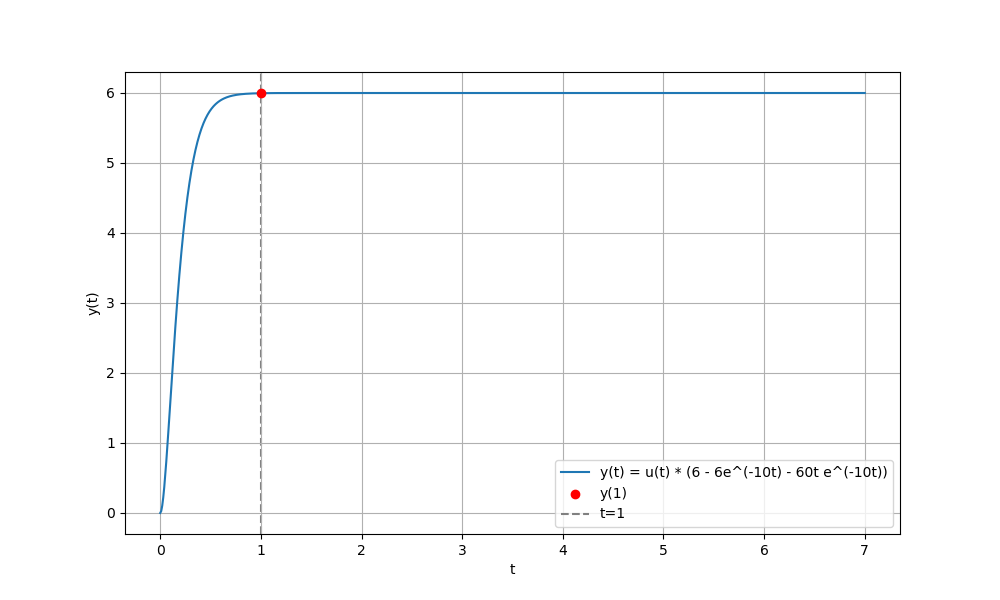
\includegraphics[width=\columnwidth]{fig/plot.png}

    \centering
    \caption{Plot of $y\brak t = u\brak t \brak{6-6e^{-10t}-60te^{-10t}}$}

    \label{fig:}
\end{figure}
\end{document}
